\subsection{Real Data}

We now present the results of running our algorithms on several real
datasets. In the graphs that we use, each node corresponds to a single
product in the catalog of a merchant and the edges connect similar
products. For each product up to 50 most similar products were
selected by a proprietary algorithm of BloomReach that uses text-based
features such as keywords, color, brand, gender (where applicable) as
well as user browsing patterns to determine the similarity between
pairs of products. Such algorithms are commonly used in e-commerce websites
such as Amazon, Overstock, eBay etc to display the most related products 
to the user when they are browsing a specific product. \vs

Two of the client merchants of BloomReach presented here had
moderate-sized relation graphs with about $10^5$ vertices and $10^6$
input edges (candidate recommendations); the remaining merchants (3, 4
and 5) have on the order of $10^6$ vertices and $10^7$ input edges
between them.  We estimated an upper bound on the optimum solution by
taking the minimum of $|L|c/a$ and the number of vertices in $R$ of
degree at least $a$. Figures~\ref{fig:real_a=1},~\ref{fig:real_a=2}
and~\ref{fig:real_a=3} plot the average of the optimality percentage
of the sampling, greedy and partition algorithms across all the
merchants respectively. Note that we could only run the partition
algorithm for the first two merchants due to memory constraints. \vs

\begin{figure}[h]
\centering
\begin{minipage}[h]{0.48\textwidth}
\centering
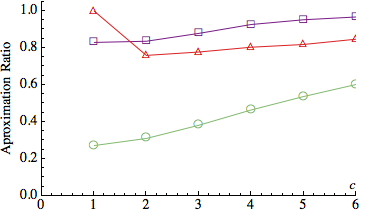
\includegraphics[width=0.99\textwidth]{images/real_a=1_new.png}

\caption{Solution quality for the $(c, 1)$-recommendation subgraph problem in retailer data}
\label{fig:real_a=1}
\end{minipage}

\hspace{0cm}
\begin{minipage}[h]{0.48\textwidth}
\centering
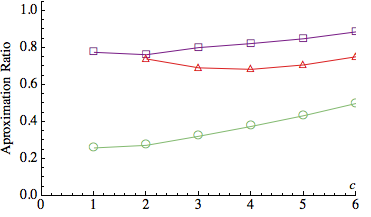
\includegraphics[width=0.99\textwidth]{images/real_a=2_new.png}

\caption{Solution quality for the $(c, 2)$-recommendation subgraph problem in retailer data}
\label{fig:real_a=2}
\end{minipage}

\hspace{0cm}
\begin{minipage}[h]{0.48\textwidth}
\centering
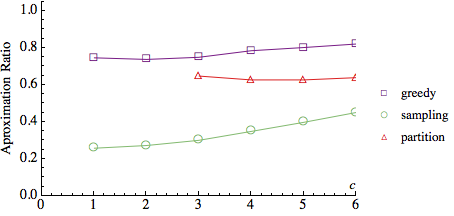
\includegraphics[width=0.99\textwidth]{images/real_a=3_new.png}

\caption{Solution quality for the $(c, 3)$-recommendation subgraph problem in retailer data}
\label{fig:real_a=3}
\end{minipage}
\vspace{-.3cm}
\end{figure} \vs

From these results, we can see that that greedy performs exceptionally
well when $c$ gets even moderately large.  For the realistic value of
$c=6$, the greedy algorithm produced a solution that was 85\% optimal
for all the merchants we tested. For several of the merchants, its
results were almost optimal starting from $a=2$. \vs

The partition method is also promising, especially when the $a$ value
that is targeted is low. Indeed, when $a=1$ or $a=2$, its performance
is comparable or better than greedy, though the difference is not as pronounced as
it is in the simulations. However, for larger values of $a$ the partition
algorithm performs worse. 

The sampling algorithm performs mostly well on real data,
especially when $c$ is large. It is typically worse than
greedy, but unlike the partition algorithm, its performance improves
dramatically as $c$ becomes larger, and its performance does not worsen
as quickly when $a$ gets larger. Therefore, for large $c$ 
sampling becomes a viable alternative to greedy mainly in cases where the
linear memory cost of the greedy algorithm is too prohibitive.
